\documentclass[a4paper,10pt]{scrartcl}

\usepackage[utf8]{inputenc}
\usepackage[ngerman]{babel}
\usepackage[T1]{fontenc}
\usepackage{amsmath}
\usepackage[section]{placeins}
\usepackage{graphicx}
\usepackage{esvect}

\title{Praktikum B Vorbereitung zu Versuch "lb"}
\author{Leon Machtl und Raphael Lehner}
\date{06.02.2020}

\begin{document}
	\maketitle
	\tableofcontents
	\newpage
	
	\section{Einleitung zum Versuch}
	
	Die Beugung, die auch als Diffraktion bezeichnet wird, ist die Ablenkung von Wellen an einem beliebigen Objekt. Ein Effekt der Beugung ist, dass sich die Lichtwelle auch in Schattenbereiche des Hindernisses ausbreiten kann, also in Bereiche, die eigentlich auf geradem Weg durch das Objekt verdeckt werden würden. Beugung betrifft jede Art physikalischer Wellen, bei Schall und Wasser ist sie jedoch besonders deutlich erkennbar. Betrachtet man Lichtwellen, stellt die Beugung einen Faktor dar, durch den das Auflösungsvermögen begrenzt wird (zum Beispiel in Teleskopen). Die Fresnelsche Zonenplatte und Begungsgitter sind Beispiele für eine gezielte Ausnutzung der Beugung. Die Entstehung der Beugung lässt sich mit Hilfe des Huygenschen Prinzips erklären, welches besagt, dass sich jeder Punkt einer Wellenfront als Ausgangspunkt einer Elementarwelle betrachten lässt und sich somit die weiteren Wellenfronten durch die Überlagerung dieser Elementarwellen ergeben. Die Elementarwellen beschreiben dabei einen Kreis. Betrachtet man einen unendlich dünnen Spalt, kann sich nur noch eine einzige Elementarwelle bilden, und somit entstehen keine Wellenfronten durch Superposition. Somit erhält man durch sehr kleine Spalte also Punktlichtquellen. Dadurch kommt es zu interessanten Phänomenen wie Interferenz- und Beugungsmustern. In den nachfolgenden Rechnungen wird monochromatisches und kohärentes Licht angenommen, um sie zu erleichtern.
	
	\subsection{Wichtige Formeln}
		\subsubsection{Einfachspalt}
			Lage der Minima: \(sin(\Phi_{k,min})=\frac{\lambda}{b}k\) \\
			Lage der Maxima: \(sin(\Phi_{k,max})=\frac{\lambda}{b}(k+\frac{1}{2})\)\\
			Hauptmaximum: \(\Phi_{0,max}=0\)\\
			wobei \(k=1,2,3,...\) Beugungsordnung heißt.
			
		\subsubsection{Doppelspalt}
			Lage der Minima II. Klasse: \(sin(\Psi_{m,min})=\frac{\lambda}{d}(m+\frac{1}{2})\)\\
			Maxima II. Klasse: \(sin(\Psi_{m,max})=\frac{\lambda}{d}m\)\\
			mit \(m=0,1,2,3,..\)
			
		\subsubsection{N-fach Spalt und Gitter}
			Minima und Maxima I. und II. Klasse bleiben an den gleichen Stellen, die Extremstellen II. Klasse werden jedoch schmaler, dazwischen bilden sich \(N-2\) schwächere Nebenmaxima.\\
			Intensität des gebeugten Lichtes: 
			\begin{align*}
			I(\Phi)=\frac{sin^{2}(\frac{\pi b}{\lambda}sin(\Phi))}{(\frac{\pi b}{\lambda}sin(\Phi))^{2}}\frac{sin^{2}(\frac{N\pi d}{\lambda}sin(\Phi))}{(sin(\frac{N\pi d}{\lambda}sin(\Phi)))^{2}}
			\end{align*}
		
		


	\section{Fragen zur Vorbereitung}
		\subsection{Frage 1}
		Nehmen Sie an, die Beugung findet nicht in Luft (\(n\approx1\), sondern in Wasser statt (\(n>1\)). Wie
		ändert sich das Beugungsbild?\\
		\\
		Wie in dem Abschnitt über wichtige Formeln aufgeführt, hängt die Lage der Extrema sowohl beim Einfach- als auch beim Doppelspalt von der Wellenlänge ab. Für die Wellenlänge in einem Medium \(n\) gilt: 
		\begin{align*}
		\lambda '= \frac{\lambda_{0}}{n}
		\end{align*}
		Somit gilt für die Luft ungefähr
		\begin{align*}
		\lambda = \lambda_{0}
		\end{align*}
		Im Wasser jedoch
		\begin{align*}
		\lambda '= \frac{\lambda_{0}}{n}
		\end{align*}
		mit \(n>1\), somit ist Wellenlänge im Wasser kleiner als in der Luft. Betrachtet man nun die Formeln aus dem Vorbereitungsteil im Kapitel Einfachspalt, so sieht man sofort, dass die Extrema zusammenrücken.
		
		\subsection{Frage 2}
		Es werde zuerst das Beugungsbild eines Doppelspalts fotografisch aufgenommen; auf einem
		gleichartigen Film werden dann nacheinander die Beugungsfiguren beider Einzelspalte auf
		demselben Film aufgenommen. Insgesamt werden beide Filme gleich lange belichtet. Vergleichen
		Sie die Beugungsbilder miteinander. Erklären Sie Gleichheit oder Ungleichheit.\\
		\\
		Werden zwei Einzelspalte überlagert, so erhält man keine einfache Addition der Beugungsfiguren als Intensitätsverteilung, da durch die Interferenz des Lichts beider Spalte ein Interferenzmuster entsteht, welches hochfrequente Modulierungen mit Extrema II. Klasse aufweist, welche bei den Beugungsfiguren der einzelnen Spalte nicht auftauchen. Die Einhüllende des Doppelspalt Bildes jedoch entspricht der Überlagerung zweier Einzelspalt Bilder.

\FloatBarrier
			\begin{figure}[h]
\centering
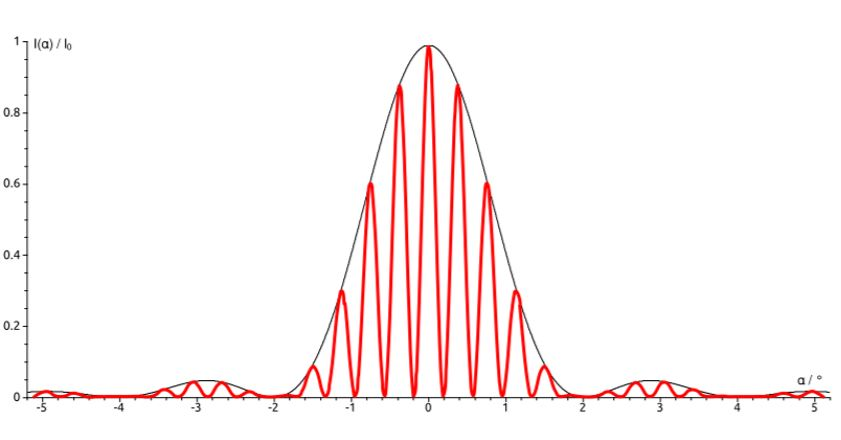
\includegraphics[width=0.7\textwidth]{./Bilder/lb1}

\end{figure}
\FloatBarrier
		\subsection{Frage 3}
		Nehmen Sie an, bei einem Doppelspalt werden die beiden Spalte jeweils von verschiedenen
		Lasern beleuchtet. Wie würde sich das Beugungsbild gegenüber dem üblichen Experiment ändern?\\
		\\
		Es gibt zwei Faktoren, welche eine Änderung verursachen können. Zum Einen die Phasenbeziehung: Da sich die beiden näherungsweisen Punktquellen in keiner definierten Phasenbeziehung zueinander befinden, kann sich der Mittelpunkt des Interferenzmusters am Schirm gegenüber der optischen Aschse verschieben.\\
		Der andere Faktor ist die Wellenlänge des Lichts der beiden Laser: Beistzen die beiden Laser die selbe Wellenlänge, so interferiert das Licht in gewohnter Weise, wie in den Formeln des oberen Abschnitts. Sind die beiden Wellenlängen voneinander verschieden, so ergibt sich eine Überlagerung zweier Einfachspaltbilder mit unterschiedlichem \(\lambda\).
		

		\subsection{Frage 4}
		Nehmen Sie an, ein Laserstrahl wird durch Spiegel aufgespalten und die beiden Strahlen beleuchten je einen Spalt. Besteht ein Unterschied zu dem vorher geschilderten Fall? Wenn ja,	erklären Sie, weshalb.\\
		\\
		Da das Licht aus der gleichen Lichtquelle stammt, ist die Wellenlänge beider Strahlen identisch. Die Phasen der beiden Strahlen werden jedoch durch die Reflexion und unterschiedliche Laufzeiten phasenverschoben, wodurch sich, wie in der Aufgabe zuvor eine Verschiebung des Interferenzmusters gegenüber der optischen Achse ergibt.

		\subsection{Frage 5}
		Wie ändert sich das Beugungsbild eines Spalts, wenn dieser statt mit einem Laser mit Licht
		einer Hg-Dampflampe beleuchtet wird?\\
		\\
		Quecksilberdampflampen weisen ein Linienspektrum auf, das Spektrum besitzt also mehrere scharfe Peaks. Für jeden dieser Peaks entsteht nun beim Doppelspalt je ein Interferenzmuster. Diese verschiedenen Interferenzmuster überlagern sich nun gemäß der Superposition zu einem einzelnen Muster, welches aufgrund der Beschaffenheit des menschlichen Auges regenbogenartig erscheint.
		
\FloatBarrier
			\begin{figure}[h]
\centering
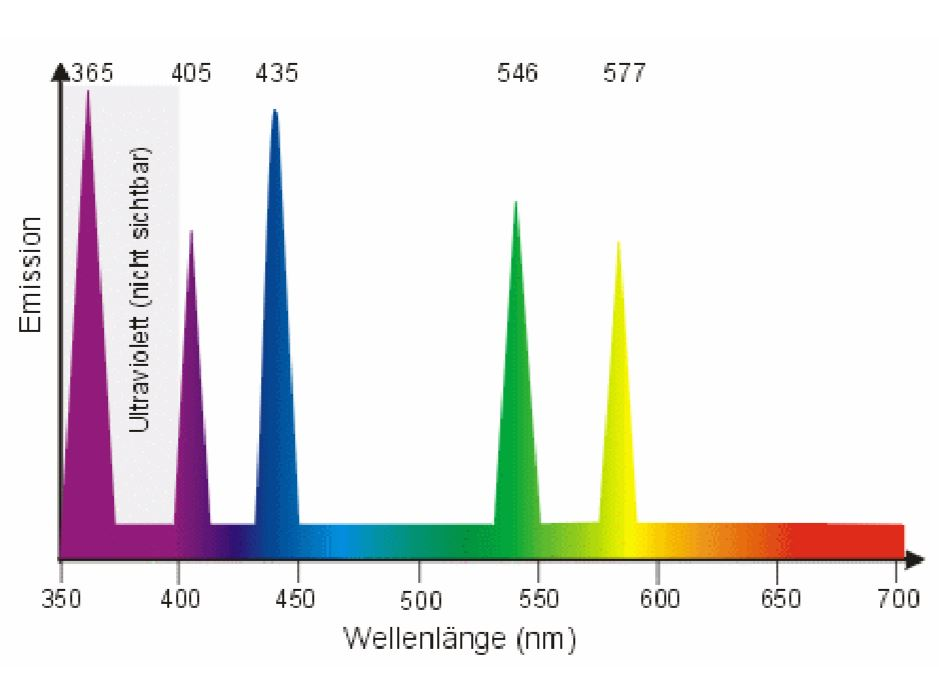
\includegraphics[width=0.7\textwidth]{./Bilder/lb2}

\end{figure}
\FloatBarrier
		\subsection{Frage 6}
		Was unterscheidet Fraunhofer- und Fresnel-Beugung?\\
		\\
		\begin{itemize}
			\item Fraunhoferbeugung
			\begin{itemize}
				\item Spalt durch parallele Lichtstrahlen beleuchtet
				\item Näherungsweise im Fernfeld einer Punktlichtquelle der Fall
				\item Bei Fraunhoferbeugung betrachtet man also das Fernfeld
			\end{itemize}
			\item Fresnelbeugung
			\begin{itemize}
				\item Lichtstrahlen fallen nicht parallel auf den Spalt
				\item Winkel nicht vernachlässigbar
				\item Die Fresnelbeugung betrachtet also das Nahfeld, also eine endliche Entfernung
			\end{itemize}
		\end{itemize}

\FloatBarrier
			\begin{figure}[h]
\centering
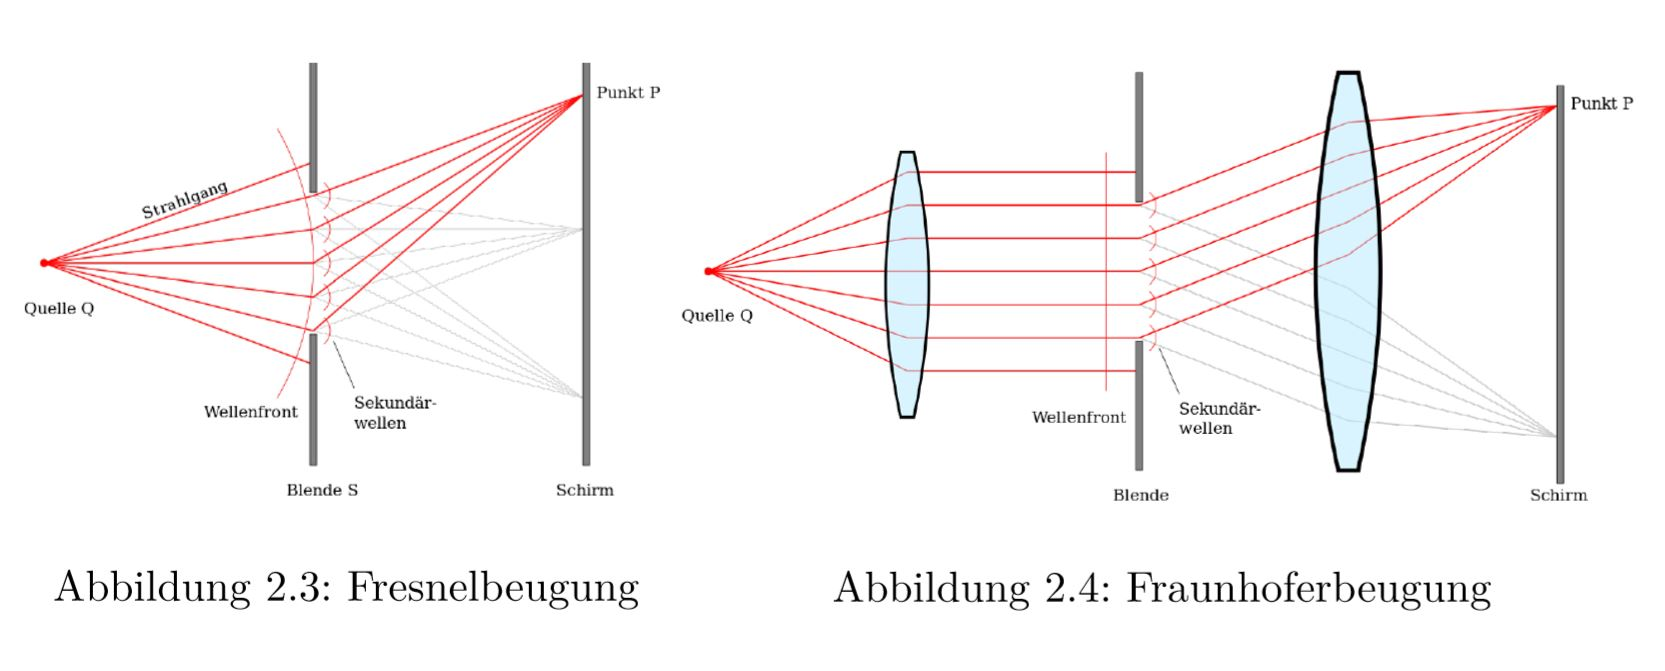
\includegraphics[width=0.7\textwidth]{./Bilder/lb3}

\end{figure}
\FloatBarrier
			
\subsection{Frage 7}
Leiten Sie für den Einfachspalt die Formel \(I(\phi)=I_{0}sinc^{2}(\frac{\Theta}{2})\) mit \(\Theta = \frac{2\pi}{\lambda}bsin(\phi)\) und \(I_{0}=I(\phi=0)\) für die Intensitätsverteilung in Abhängigkeit vom Beugungswinkel \(\phi\) ab. Berechnen Sie das Intensitätsverhältnis \(I(\phi_{k,max})/I(\phi=0)\) für die erste (\(k=1\)) und zweite (\(k=2\)) Beugungsordnung.\\
\\
Unter der Annahme, dass die Spaltanordnung komplett zweidimensional ist, es also nur eine Breite, aber keine Höhe gibt, ergibt sich mit der Fraunhoferbeugung das Integral:
\begin{align*}
E(\beta)\propto\int_{-\infty}^{\infty}\Omega(x)exp(-ik\beta x)dx
\end{align*} 
mit der Wellenzahl \(k\), \(\beta =sin(\phi)\) und der Koordinate x und \(\Omega (x)=1\) falls \(-\frac{b}{2}\leq x \leq \frac{b}{2}\) und \(\Omega (x)=0\) sonst. Somit folgt
\begin{align*}
\int_{-\infty}^{\infty}\Omega(x)exp(-ik\beta x)dx=\int_{-\frac{b}{2}}^{\frac{b}{2}}exp(-ik\beta x)dx=\frac{1}{-ik\beta}[exp(-ik\beta\frac{b}{2})-exp(ik\beta\frac{b}{2})]
\end{align*}
\begin{align*}
=\frac{2sin(k\beta \frac{b}{2})}{k\beta}=\frac{sin(k\beta\frac{b}{2})}{\frac{k\beta}{2}}
\end{align*}
Es gilt \(I\propto EE^{*}=|E|^{2}\), somit folgt aus der obigen Rechnung:
\begin{align*}
|E|^{2}\propto\frac{sin^{2}(k\beta\frac{b}{2})}{(\frac{k\beta}{2})^{2}}
\end{align*}
Für die Berechnung von \(I(\beta=0)\) nutzt man die Regel von l'Hopital:

\begin{align*}
I(\beta=0)=\lim\limits_{\beta \rightarrow 0}{\frac{sin^{2}(k\beta\frac{b}{2})}{(\frac{k\beta}{2})^{2}}}=\lim\limits_{\beta \rightarrow 0}{\frac{[cos^{2}(\frac{k\beta b}{2})-sin^{2}(\frac{k\beta b}{2})]k^{2}\frac{b^{2}}{4}}{\frac{k^{2}}{4}}=b^{2}}
\end{align*}
Somit folgt 
\begin{align*}
\frac{I(\beta)}{I_{0}}=\frac{sin^{2}(k\beta\frac{b}{2})}{(\frac{k\beta b}{2})^{2}}=sinc^{2}(k\beta \frac{b}{2})=sinc^{2}(\frac{2\pi}{\lambda}sin(\phi)\frac{b}{2})=sinc^{2}(\frac{\Theta}{2})
\end{align*}

Damit sieht man sofort: 

\begin{align*}
I(\beta)=I_{0}sinc^{2}(\frac{\Theta}{2})
\end{align*}

was zu zeigen war.

\begin{align*}
sin(\Phi_{1,max})=\frac{\lambda}{b}(1+\frac{1}{2})=\frac{3\lambda}{2b}
\end{align*}
daraus folgt 
\begin{align*}
\Theta=3\pi
\end{align*}
also
\begin{align*}
\frac{I_{1,max}}{I_{0}}=sinc^{2}(\frac{3\pi}{2})=\frac{4}{9\pi^{2}}=0,045
\end{align*}
\begin{align*}
sin(\Phi_{2,max})=\frac{\lambda}{b}(2+\frac{1}{2})=\frac{5\lambda}{2b}
\end{align*}
\begin{align*}
\Theta=5\pi
\end{align*}
\begin{align*}
\frac{I_{2,max}}{I_{0}}=\frac{4}{25\pi^{2}}=0,016
\end{align*}
\FloatBarrier
			\begin{figure}[h]
\centering
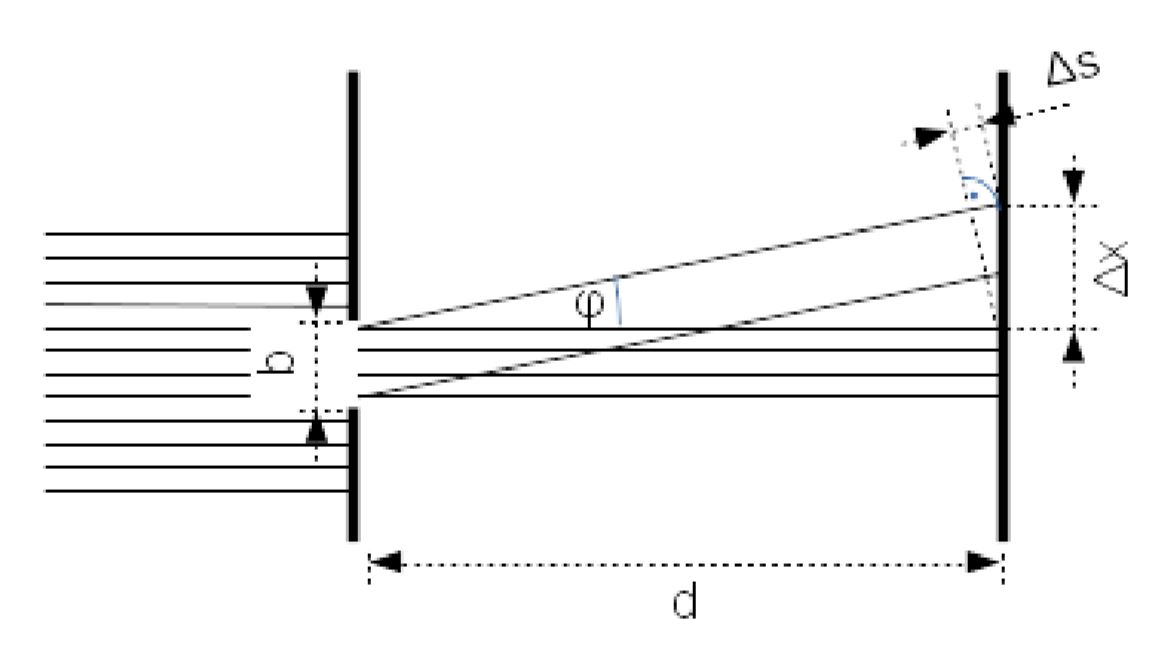
\includegraphics[width=0.7\textwidth]{./Bilder/lb4}

\end{figure}
\FloatBarrier

\subsection{Frage 8}
Verifizieren Sie für den Doppelspalt den Ausdruck\(I(\phi)=4I_{0}sinc^{2}(\frac{\Theta}{2})cos^{2}(\frac{\delta}{2})\) mit \(\Theta=\frac{2\pi}{\lambda}bsin(\phi)\) und \(\delta=\frac{2\pi}{\lambda}dsin(\phi)\) und \(I_{0}\) aus Aufgabe 7. Begründen Sie anschaulich das Auftreten des Faktors 4 und berechnen Sie die Intensität des
ersten Nebenmaximums \(m=1\) relativ zum nullten in Abhängigkeit von Spaltbreite b und
Spaltabstand d. Für welches Verhältnis d/b fällt das fünfte Nebenmaximum mit dem ersten
Haupt-Minimum zusammen?\\
\\
Rechne wie in Aufgabe 7 mit \(\Omega_{DS}=\Omega_{1}(x)-\Omega_{2}(x)\) wobei \(\Omega_{1}=1\) für \(-\frac{d+b}{2}\leq x\leq \frac{d+b}{2}\) und ansonsten gleich 0 ist und \(\Omega_{2}=1\) für \(-\frac{d-b}{2}\leq x \leq \frac{d-b}{2}\) und sonst gleich 0. Damit erhält man mit der Fraunhofer-Beugungstheorie:
\begin{align*}
E(\beta)=\int_{-\infty}^{\infty}(\Omega_{1}(x)-\Omega_{2}(x))exp(-ik\beta x)dx=\int_{-\frac{d+b}{2}}^{\frac{d+b}{2}}exp(-ik\beta x)dx-\int_{-\frac{d-b}{2}}^{\frac{d-b}{2}}exp(-ik\beta x)dx
\end{align*}
Dies berechnet sich wie in der Aufgabe zuvor zu
\begin{align*}
\frac{2}{k\beta}[sin(k\beta\frac{d+b}{2})-sin(k\beta \frac{d-b}{2})]=2cos(k\beta \frac{d}{2})\frac{sin(k\beta\frac{b}{2})}{\frac{k\beta}{2}}
\end{align*}
Aus \(I\propto EE^{*}=|E|^{2}\) folgt dann wieder
\begin{align*}
I\propto 4cos^{2}(k\beta \frac{d}{2})\frac{sin^{2}(k\beta\frac{b}{2})}{(\frac{k\beta}{2})^{2}}
\end{align*}

\(I_{0}=b^{2}\) nach Aufgabenstellung, somit erhält man

\begin{align*}
\frac{I_{DS}}{I_{0}}=4cos^{2}(k\beta \frac{d}{2})sinc^{2}(k\beta\frac{b}{2})
\end{align*}
Woraus sofort folgt
\begin{align*}
I_{DS}=4I_{0}cos^{2}(k\beta \frac{d}{2})sinc^{2}(k\beta\frac{b}{2})
\end{align*}
Dies ergibt mit \(k\), \(\beta\) wie oben das, was zu zeigen war.
Nun berechne Intensität für \(m=1\):
\begin{align*}
sin(\Psi_{1,max})=\frac{\lambda}{d}
\end{align*}
damit ergibt sich
\begin{align*}
\Theta=\frac{2\pi b}{d}
\end{align*}
\begin{align*}
\delta=2\pi
\end{align*}
Setzt man dies ein, erhält man die Intensität
\begin{align*}
\frac{I_{DS}}{I_{0}}=4sinc^{2}(\frac{\pi b}{d})
\end{align*}
Das erste Hauptminimum liegt bei 
\begin{align*}
sin(\Phi_{1,min})=\frac{\lambda}{b}
\end{align*}
das fünfte Nebenmaximum liegt bei
\begin{align*}
sin(\Psi_{5,max})=\frac{\lambda}{d}5
\end{align*}
fallen diese Zusammen, gilt somit:
\begin{align*}
\frac{d}{b}=5
\end{align*}
\end{document}
